\documentclass[12pt]{article}
\usepackage[a4paper, margin=1in]{geometry} 
\usepackage{graphicx} 
\usepackage{hyperref}
\usepackage{float}
\usepackage{multicol}
\usepackage{amsmath}
\usepackage[ruled]{algorithm2e}
\usepackage[font=small, labelfont=bf]{caption}

\title{Lecture Notes for \\ INF281 Basics of Bioinformatics Sequence Analysis}
\author{Takaya Saito}
\date{}

\begin{document}

\pagenumbering{arabic}
\setcounter{page}{1}

\makeatletter 
\renewcommand{\thefigure}{\arabic{section}.\arabic{figure}}
\renewcommand{\thetable}{\arabic{section}.\arabic{table}}
\makeatother

%
% PART I
%
\part{}

%
% Introduction
%
\setcounter{figure}{0}
\section{Introduction}
%\documentclass[12pt]{article}
%\usepackage[a4paper, margin=1in]{geometry} 
%\usepackage{graphicx} 
%\usepackage{hyperref}
%\usepackage{float}
%\usepackage[font=small, labelfont=bf]{caption}
%
%\begin{document}

%
% Introduction to Molecular Biology
%
\subsection{Introduction to Molecular Biology}
Molecular biology is the study of biology focusing on organisms and cells at the molecular level.

%
% Five essential facts about cells
%
\subsubsection*{Five essential facts about cells}

\textbf{1. Two primary types of cells –- eukaryotes and prokaryotes}
\begin{itemize}
\item Eukaryote: animals \& plants
\item Prokaryote: bacteria \& archaea
\end{itemize}
\begin{figure}[H]
  \centering
      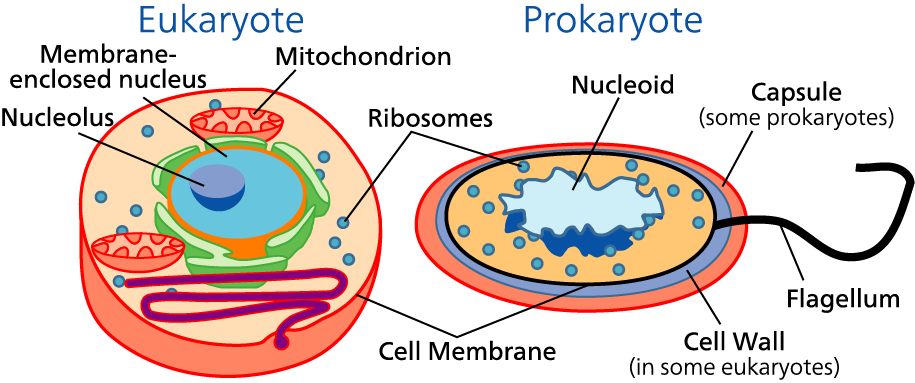
\includegraphics[width=0.75\textwidth]{fig01/prokaryote_and_eukaryote_cells.png}
  \caption{Eukaryotic and prokaryotic cells (source: \href{https://commons.wikimedia.org/wiki/File:Celltypes.svg}{Science Primer, Wikimedia Commons})}
\end{figure}

\noindent \textbf{2. Cell size –- around 1 to 100 micrometers}
\begin{itemize}
\item Cell Size and Scale: \url{http://learn.genetics.utah.edu/content/cells/scale}
\end{itemize}
\medskip  

\noindent \textbf{3. The number of cells}
\begin{itemize}
\item Prokaryotes: 1 cell
\item Human:  Estimate of 15 trillion cells
\end{itemize}
\medskip 

\noindent \textbf{4. An animal cell and cell organelles}
\begin{figure}[H]
  \centering
      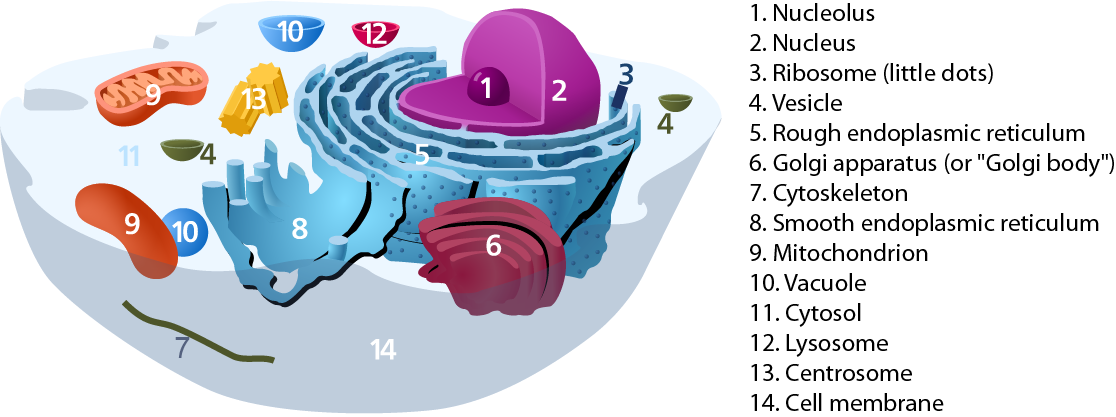
\includegraphics[width=0.75\textwidth]{fig01/animal_cells_and_organelles.png}
  \caption{An animal cell and organelles (source: \href{https://en.wikipedia.org/wiki/Organelle\#/media/File:Animal_Cell.svg}{Kelvinsong, Wikimedia Commons})}
\end{figure}

\noindent \textbf{5. Cellular processes}
\begin{itemize}
\item Cell growth, cell development, cell signaling, …
\item Example: \url{http://www.nature.com/nrg/multimedia/rnai}
\end{itemize}

%
% Central dogma of molecular biology
%
\subsubsection*{Central dogma of molecular biology}

It describes the information flow within a cell.

\begin{figure}[H]
  \centering
      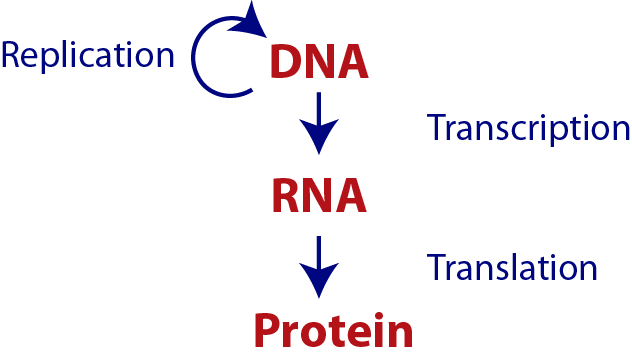
\includegraphics[width=0.75\textwidth]{fig01/central_dogma_of_molecular_biology.png}
  \caption{Central dogma of molecular biology}
\end{figure}

%
% DNA (deoxyribonucleic acid)
%
\subsubsection*{DNA (deoxyribonucleic acid)}

DNA stores genetic information. It has four different bases: cytosine (C), guanine (G), adenine (A), and thymine (T).

\begin{figure}[H]
  \centering
      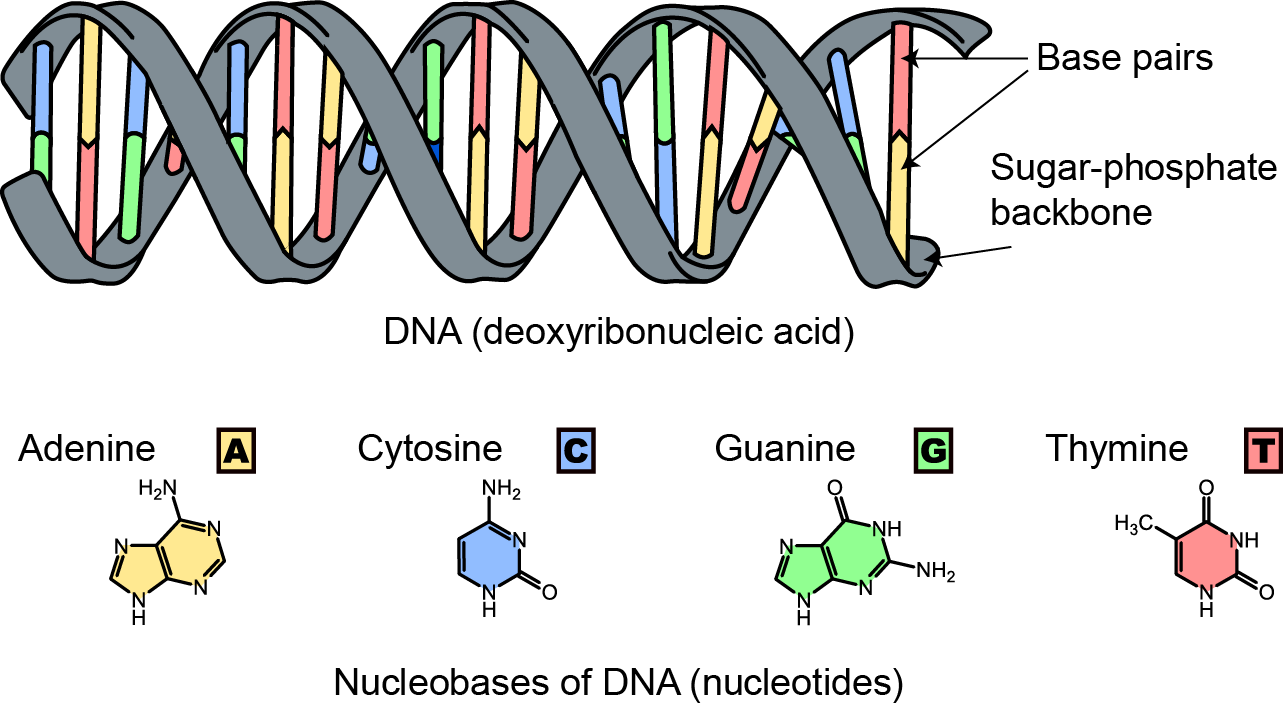
\includegraphics[width=0.5\textwidth]{fig01/dna_bases.png}
  \caption{DNA double helix and base pairs \newline (modified from the original version by \href{https://commons.wikimedia.org/w/index.php?curid=9810855}{Sponk, Wikimedia Commons})}
\end{figure} 

\noindent \textbf{Base pair matching (Watson-Crick base pair)}

\noindent Adenine (A) pairs with thymine (T), whereas cytosine (C) pairs with guanine (G).

\begin{verbatim}
DNA strand1: ACGT
             ||||
DNA strand2: TGCA
\end{verbatim}
	
%
% RNA (Ribonucleic acid)
%
\subsubsection*{RNA (Ribonucleic acid)}
RNA has various biological roles and several sub-classes. Messenger RNAs (mRNAs) convey genetic information.  It has four different bases: cytosine (C), guanine (G), adenine (A), and uracil (U).

\begin{figure}[H]
  \centering
      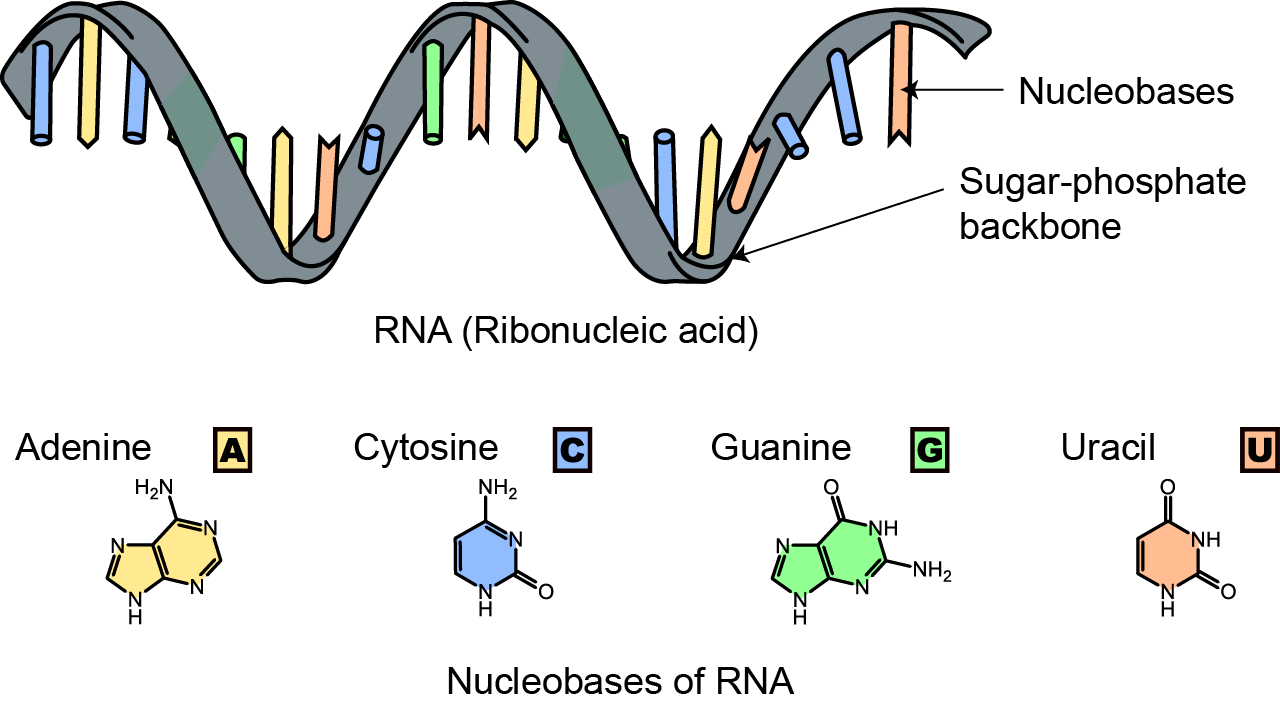
\includegraphics[width=0.5\textwidth]{fig01/rna_bases.png}
  \caption{Single strand RNA \newline (modified from the original version by \href{https://commons.wikimedia.org/w/index.php?curid=9810855}{Sponk, Wikimedia Commons})}
\end{figure}

\noindent \textbf{Transcription: mRNAs are transcribed from DNAs}

\begin{verbatim}
DNA: ACGT -------> RNA: ACGU
        Transcription
\end{verbatim}

%
% Protein
%
\subsubsection*{Protein}

Proteins are large molecules consisting of amino acids. There are 20 common amino acids.
 
\begin{figure}[H]
  \centering
      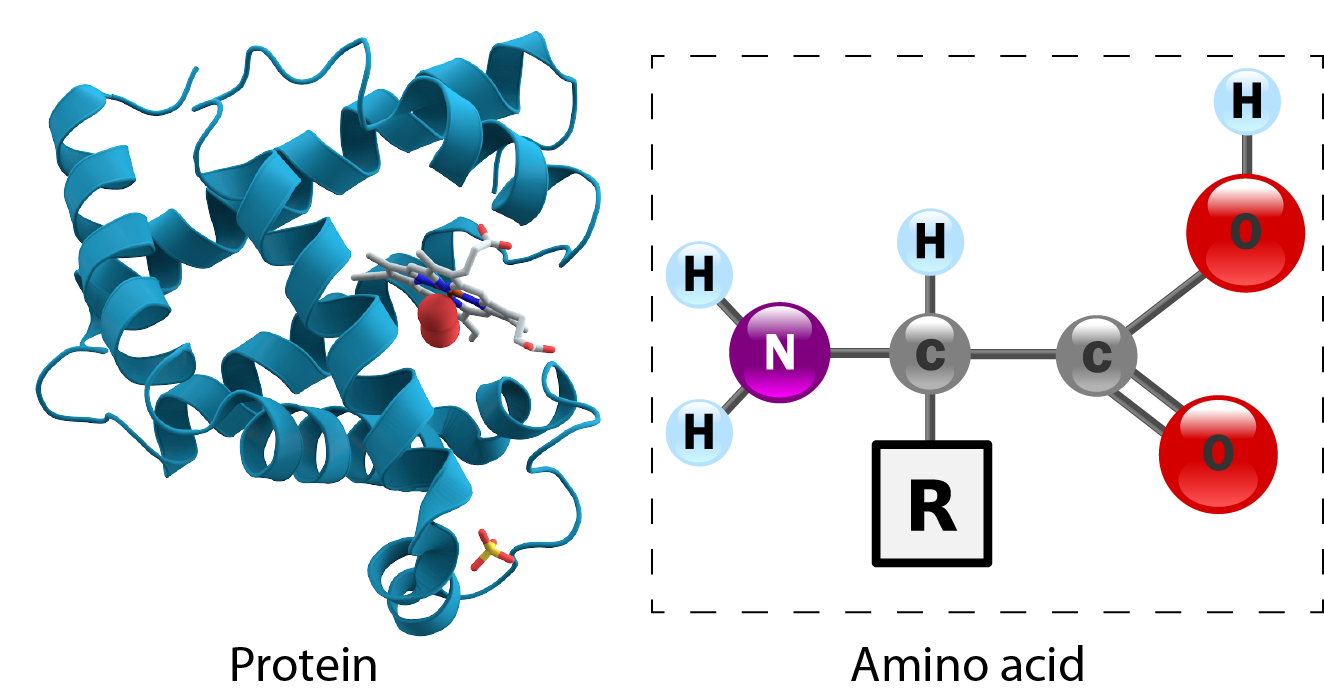
\includegraphics[width=0.6\textwidth]{fig01/protein_and_amino_acid.png}
  \caption{Protein 3D structure and amino acids \newline (sources: \href{https://en.wikipedia.org/wiki/Protein\#/media/File:Myoglobin.png}{AzaToth, Wikimedia Commons}, \href{https://en.wikipedia.org/wiki/Amino_acid\#/media/File:AminoAcidball.svg}{YassineMrabet, Wikimedia Commons})}
\end{figure}

\noindent \textbf{Translation: Amino-acids are translated from mRNAs}

\begin{verbatim}
mRNA: GUC -------> AA: Valine
        Translation
\end{verbatim}

\newpage 

\noindent \textbf{Universal genetic code}

\noindent A codon consists of three nucleic acids. Single-letter or three-letter names can be used for amino acids.

\begin{figure}[H]
  \centering
      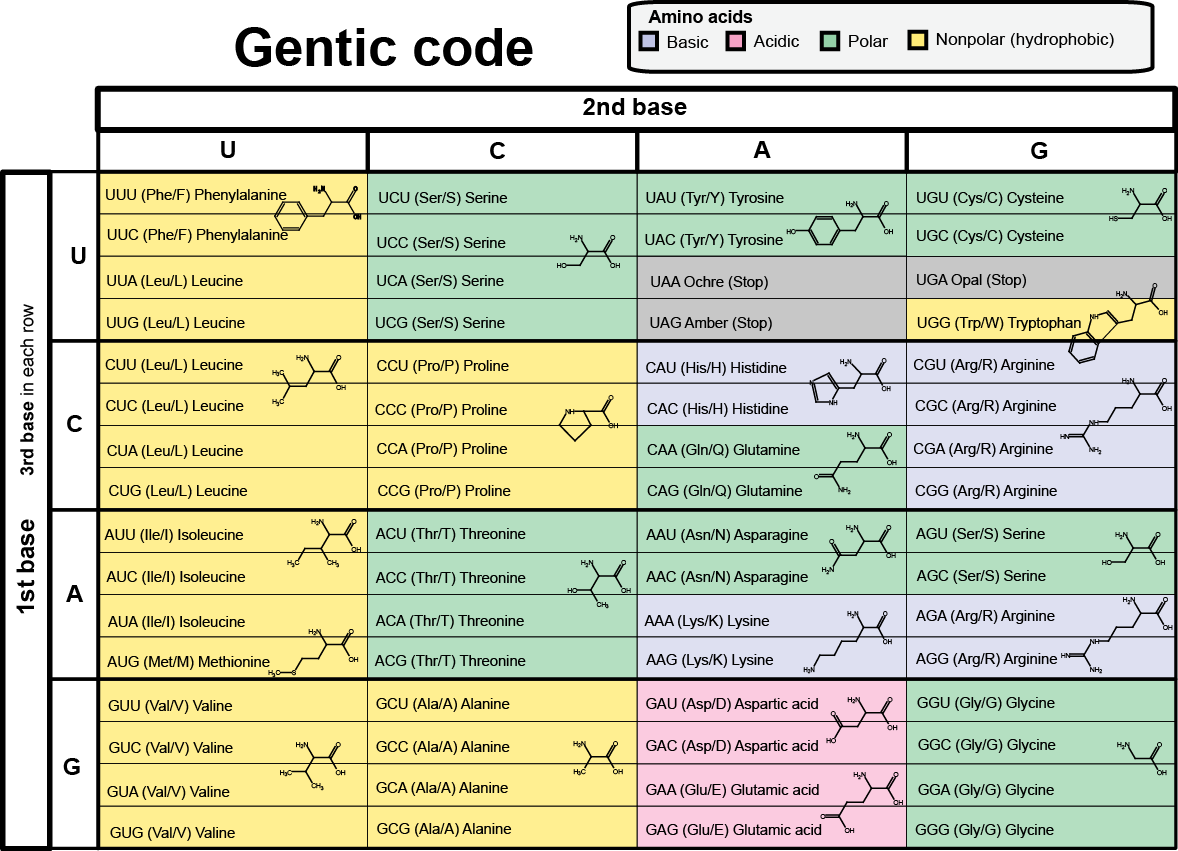
\includegraphics[width=0.7\textwidth]{fig01/genetic_code.png}
  \caption{Universal genetic code \newline (modified from the original version by \href{https://commons.wikimedia.org/wiki/File\%3ANotable_mutations.svg}{H\"aggstr\"om, Wikimedia Commons})}
\end{figure}

\noindent \textbf{Cellular functions of proteins}
\begin{itemize}
\item Enzymes: catalyze chemical reaction
\item Cell signaling: hormone (e.g. insulin), antibodies, …
\item Structural: collagen, cartilage, keratin, …
\end{itemize}

%
% Exercises 1.1
%
\subsubsection*{Exercises 1.1}
\begin{enumerate}

\item Draw a simple diagram of the central dogma of molecular biology and briefly explain the information flow of the molecules.

\item What are the DNA sequences of the opposite strand for the following DNA sequences?
\begin{verbatim}
    Seq1 CCGATT
    Seq2 TTACGC
    Seq3 ACGCGC
\end{verbatim}

\item What are the mRNA sequences transcribed from the following DNA sequences?

\item What are the polypeptide sequences translated from the following mRNA sequences? Answer them with both one-letter and three letter names.
\begin{verbatim}
    Seq1 AUGUUUUAA
    Seq2 GCAGCAAAA
\end{verbatim}
		
\end{enumerate}

%\end{document}

%\documentclass[12pt]{article}
%\usepackage[a4paper, margin=1in]{geometry} 
%\usepackage{graphicx} 
%\usepackage{hyperref}
%\usepackage{float}
%\usepackage[font=small, labelfont=bf]{caption}

%\begin{document}

%
% Introduction to Biotechnology
%
\subsection{Introduction to Biotechnology}
Biotechnology is the use of laboratory techniques to study living organism and cells. 

%
% Applications of biotechnology
%
\subsubsection*{Applications of biotechnology}
Branches of biotechnology can be explained with different colors.
\begin{itemize}
\item Red: medical processes
\item Green: agricultural processes
\item White: industrial processes
\item Blue: marine and aquatic applications
\end{itemize}

%
% Laboratory tools and equipment
%
\subsubsection*{Laboratory tools and equipment}

\begin{figure}[H]
  \centering
      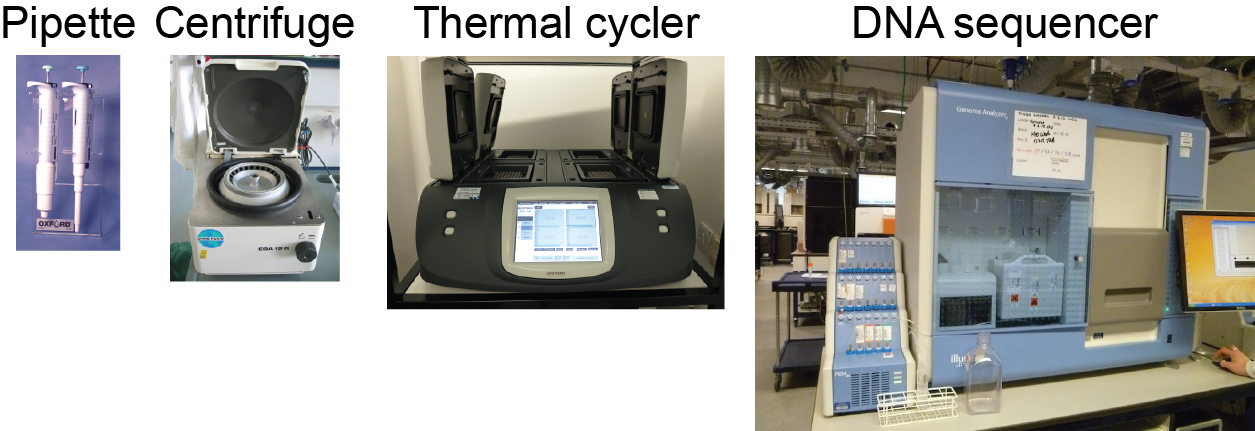
\includegraphics[width=0.5\textwidth]{fig01/lab_equipment.png}
  \caption{Pipette, centrifuge, thermal cycler, and DNA sequencer \newline (sources:  \href{https://en.wikipedia.org/wiki/Pipette\#/media/File:Single_channel_rack.jpg}{Domain}, \href{https://commons.wikimedia.org/w/index.php?curid=494}{Manske},
\href{https://commons.wikimedia.org/w/index.php?curid=20189025}{Rror}, 
\href{https://commons.wikimedia.org/w/index.php?curid=18862968}{RE73} via Wikimedia Commons)}
\end{figure}
 
%
% Human genome project
%
\subsubsection*{Human genome project}
It was a large-scale international research project to determine the whole DNA sequences of human.

\begin{itemize}
\item 1990 –- 2003
\item \$2.7 billion
\end{itemize}

%
% Next generation sequencing
%
\subsubsection*{Next generation sequencing}
Sequence technologies have been rapidly advanced since the human genome project.

Example: sequence a whole human genome with Illumina HiSeq X Ten.
\begin{itemize}
\item One day
\item \$1000
\end{itemize}

%
% Protein sequencing
%
\subsubsection*{Protein sequencing}
Proteins are generally more studied than DNAs and RNAs, but the whole proteome is generally harder to analyze than the whole genome. MS (mass-spectrometry) based technologies are widely used to sequence proteins.

\begin{figure}[H]
  \centering
      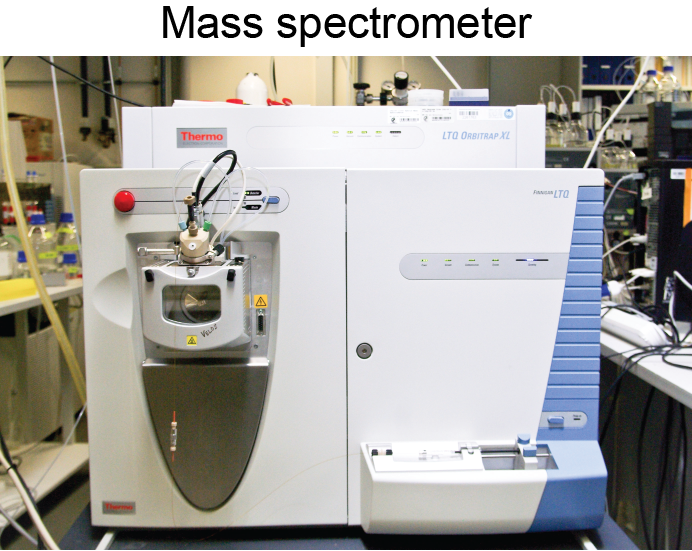
\includegraphics[width=0.25\textwidth]{fig01/mass_spectrometer.png}
  \caption{Orbitrap mass spectrometer (source: \href{https://commons.wikimedia.org/w/index.php?curid=18691799}{Wi\`{o}rkiewicz, Wikimedia Commons})}
\end{figure}
 
%\end{document}

%\documentclass[12pt]{article}
%\usepackage[a4paper, margin=1in]{geometry} 
%\usepackage{graphicx} 
%\usepackage{hyperref}
%\usepackage{float}
%\usepackage[font=small, labelfont=bf]{caption}
%
%\begin{document}

%
% Bioinformatics in INF281
%
\subsection{Bioinformatics in INF281}
Bioinformatics uses computational approaches to solve problems in life sciences. It is based on computer science.

%
% Similar or almost equivalent disciplines
%
\subsubsection*{Similar or almost equivalent disciplines}
\begin{itemize}
\item Biostatistics
\item Biophysics
\item Systems biology
\item Computational biology
\end{itemize}

%
% Not much related with bioinformatics
%
\subsubsection*{Not much related with bioinformatics}
\begin{itemize}
\item Health informatics
\item Forensic science
\end{itemize}

%
% Scope of INF281
%
\subsubsection*{Scope of INF281}
We mainly cover the following fields of bioinformatics in this course.
\begin{itemize}
\item Pairwise alignment
\item Database search
\item Statistical evaluation
\item Multiple alignment
\item Phylogenetic tree
\item Scoring scheme
\item Sequence patterns
\end{itemize}

%
% Popular bioinformatics programs
%
\subsubsection*{Popular bioinformatics programs}
BLAST and ClustalW are popular tools for sequence analysis.
\begin{itemize}
\item BLAST: a program for database search

URL: \url{http://blast.ncbi.nlm.nih.gov}

\item ClustalW: a program for multiple alignments

URL: \url{http://www.ch.embnet.org/software/ClustalW.html}

\end{itemize}

\begin{table}[!ht]
\scriptsize

\begin{tabular}{l p{10cm} r}
Rank & Title& Times cited \\
\hline
1 & Protein measurement with the folin phenol reagent & 305148 \\
2 & Cleavage of structural proteins during the assembly of the head of bacteriophage T4 & 213005 \\
3 & A rapid and sensitive method for the quantitation of microgram quantities of protein utilizing the principle of protein-dye binding & 155530 \\
4 & DNA sequencing with chain-terminating inhibitors & 65335 \\
5 & Single-step method of RNA isolation by acid guanidinium thiocyanate-phenol-chloroform extraction & 60397 \\
6 & Electrophoretic transfer of proteins from polyacrylamide gels to nitrocellulose sheets: procedure and some applications & 53349 \\
7 & Development of the Colle-Salvetti correlation-energy formula into a functional of the electron density & 46702 \\
8 & Density-functional thermochemistry. III. The role of exact exchange & 46145 \\
9 & A simple method for the isolation and purification of total lipides from animal tissues & 45131 \\
\textbf{10} & \textbf{Clustal W}: improving the sensitivity of progressive multiple sequence alignment through sequence weighting, position-specific gap penalties and weight matrix choice & 40289 \\
11 & Nonparametric estimation from incomplete observations & 38600 \\
\textbf{12} & \textbf{Basic local alignment search tool} & 38380 \\
13 & A short history of SHELX & 37978 \\
\textbf{14} & \textbf{Gapped BLAST and PSI-BLAST}: A new generation of protein database search programs & 36410 \\
15 & A revised medium for rapid growth and bio assays with tobacco tissue cultures & 36132 \\
\end{tabular}
\caption{The 15 most cited papers of all time \newline (The top 100 papers, Van Noorden, Maher, and Nuzzo, \textit{Nature}, 2014)}
\end{table}

%\end{document}


\end{document}


